\documentclass[12pt, letterpaper]{article}
\usepackage[margin=1in]{geometry}
\usepackage[T1]{fontenc}
\usepackage{lmodern}
\usepackage{cmap}
\usepackage[utf8]{inputenc}
\usepackage{amsmath, amssymb, amsthm}
\usepackage{mathtools}
\usepackage{enumitem}
\usepackage{booktabs}
\usepackage{xcolor}
\usepackage{titlesec}
\usepackage{parskip}
\usepackage{hyperref}
\usepackage{fancyhdr}
\usepackage{tcolorbox}
\usepackage{graphicx}
\usepackage{caption}
\tcbuselibrary{skins, breakable}

\definecolor{darkblue}{RGB}{15,55,115}
\definecolor{midblue}{RGB}{30,100,180}
\definecolor{theorybg}{RGB}{245,250,255}
\definecolor{questionbg}{RGB}{255,252,240}
\definecolor{evencolor}{RGB}{60,0,100}

\hypersetup{colorlinks=true,linkcolor=darkblue,urlcolor=midblue,
  pdftitle={Kurlat --- A Course in Modern Macroeconomics --- Complete Solutions, Chapters 10--11}}

\setlength{\headheight}{14pt}
\pagestyle{fancy}
\fancyhf{}
\renewcommand{\headrulewidth}{0.4pt}
\fancyhead[L]{\small\textcolor{darkblue}{\textit{Kurlat --- A Course in Modern Macroeconomics}}}
\fancyhead[R]{\small\textcolor{darkblue}{\thepage}}
\fancyfoot[C]{\small\textcolor{gray}{Complete Solutions --- Chapters 10--11}}

\titleformat{\section}[block]
  {\large\bfseries\color{darkblue}}{}{0pt}{}
  [\vspace{2pt}\color{darkblue}\rule{\textwidth}{1.5pt}\vspace{4pt}]

\titleformat{\subsection}[block]
  {\normalsize\bfseries\color{midblue}}{}{0pt}{}
  [\vspace{1pt}\color{midblue}\rule{0.5\textwidth}{0.8pt}\vspace{3pt}]

\tcbset{
  theorybox/.style={
    enhanced,breakable,colback=theorybg,colframe=darkblue,
    fonttitle=\bfseries\small\color{darkblue},boxrule=0.5pt,arc=3pt,
    left=6pt,right=6pt,top=4pt,bottom=4pt,title={Key Theory},
  },
  questionbox/.style={
    enhanced,breakable,colback=questionbg,colframe=gray!60,
    fonttitle=\bfseries\small\color{gray!60!black},boxrule=0.4pt,arc=2pt,
    left=6pt,right=6pt,top=4pt,bottom=4pt,title={\textit{Question}},
  },
  oddbox/.style={
    enhanced,breakable,colback=white,colframe=darkblue,
    attach boxed title to top left={yshift=-2mm,xshift=6mm},
    boxed title style={colback=darkblue,colframe=darkblue,arc=2pt,
      boxrule=0pt,left=6pt,right=6pt,top=3pt,bottom=3pt},
    fonttitle=\bfseries\large\color{white},
    boxrule=0.8pt,arc=3pt,
    left=8pt,right=8pt,top=10pt,bottom=6pt,
  },
  evenbox/.style={
    enhanced,breakable,colback=white,colframe=evencolor,
    attach boxed title to top left={yshift=-2mm,xshift=6mm},
    boxed title style={colback=evencolor,colframe=evencolor,arc=2pt,
      boxrule=0pt,left=6pt,right=6pt,top=3pt,bottom=3pt},
    fonttitle=\bfseries\large\color{white},
    boxrule=0.8pt,arc=3pt,
    left=8pt,right=8pt,top=10pt,bottom=6pt,
  },
  databox/.style={
    enhanced,breakable,colback=gray!8,colframe=gray!55,
    fonttitle=\bfseries\small\color{gray!60!black},boxrule=0.4pt,arc=2pt,
    left=6pt,right=6pt,top=4pt,bottom=4pt,title={Numerical exercise --- see the companion code},
  },
  trapbox/.style={
    enhanced,breakable,colback=red!4,colframe=red!45!black,
    fonttitle=\bfseries\small\color{white},boxrule=0.4pt,arc=2pt,
    coltitle=white,
    left=6pt,right=6pt,top=4pt,bottom=4pt,title={Where this goes wrong},
  },
}

\newcommand{\pd}[2]{\dfrac{\partial #1}{\partial #2}}
\newcommand{\dd}[2]{\dfrac{d #1}{d #2}}
\newcommand{\MRS}{\mathrm{MRS}}
\newcommand{\MRT}{\mathrm{MRT}}
\newcommand{\MU}{\mathrm{MU}}
\newcommand{\Var}{\mathrm{Var}}
\newcommand{\Cov}{\mathrm{Cov}}
\newcommand{\E}{\mathrm{E}}
\newcommand{\MPK}{\mathrm{MPK}}
\newcommand{\MPL}{\mathrm{MPL}}
\newcommand{\stst}{^{\ast}}

\setlist[enumerate,1]{label=(\alph*),itemsep=6pt,parsep=2pt}
\setlist[enumerate,2]{label=(\roman*),itemsep=3pt}

\newcommand{\mD}{m^{D}}
\newcommand{\Ms}{M^{S}}
\newcommand{\MBase}{M^{B}}

\begin{document}

%======================================================================
% TITLE PAGE
%======================================================================
\begin{titlepage}
\centering
\vspace*{2.5cm}
{\Huge\bfseries\color{darkblue} A Course in Modern Macroeconomics\par}
\vspace{6pt}
{\large Pablo Kurlat (2020)\par}
\vspace{1.4cm}
{\LARGE\bfseries Complete Solutions\par}
\vspace{6pt}
{\LARGE\bfseries Chapters 10--11 --- Money and Inflation\par}
\vspace{1.2cm}
{\large All fourteen end-of-chapter problems, 10.1--10.5 and 11.1--11.9 (pp.~202--222)\par}
\vspace{2cm}

\begin{tcolorbox}[theorybox,title={What is in this file},width=0.86\textwidth]
\small
Every problem carries the full question text, a step-by-step solution with no skipped
algebra, an economic reading of the result, and a verification. Numerical answers are
reproduced by the companion scripts in \texttt{Resolucao/kurlat\_ch10-11\_codigo/}, which
check each analytical formula against an independent computation (simulated deposit
chains, direct minimisation, finite differences, backward-solved price paths, root finding)
and abort on any mismatch.

\smallskip
Problems are grouped by \textbf{topic}, not by number, following the order of the
chapters' own sections. Blue boxes are odd-numbered problems, purple boxes even.

\smallskip
Lista~6 of the course is built on these two chapters; where a result overlaps
(Baumol--Tobin demand, $\eta=\tfrac12$, $\pi=\mu-\eta g$) it is derived the same way and
gives the same numbers as \texttt{lista6\_resolucao.tex}.
\end{tcolorbox}

\vfill
{\small MPE Insper --- Macroeconomia I --- 2026, 3\textordmasculine{} trimestre\par}
\end{titlepage}

\tableofcontents
\newpage

%======================================================================
\section{Chapter 10 \quad Money}
%======================================================================

\begin{tcolorbox}[theorybox,title={Chapter 10 Overview}]
\textbf{Supply.} The Central Bank controls the \emph{monetary base} (currency plus
reserves) directly. M1 (currency plus checking deposits) is created jointly with the
banking system. If banks hold exactly the required fraction $\rho$ of deposits as reserves
and the public holds a fraction $\chi$ of its M1 as cash, one unit of new base becomes
\[
\omega\equiv\frac{\Delta\text{M1}}{\Delta\text{Base}}=\frac{1}{\rho+\chi-\rho\chi}
\qquad(10.3.1)
\]
units of M1. The formula relies on banks lending out every excess reserve, which is true only
when reserves pay less than loans.

\smallskip
\textbf{Demand (Baumol--Tobin).} A household spends $pY$ evenly over the period and pays a
fixed real cost $F$ per trip to the bank. With $N$ trips its average balance is
$M=pY/2N$ (10.4.1); minimising $pFN+i\,pY/2N$ (10.4.2) gives
\[
N=\sqrt{\frac{iY}{2F}}\quad(10.4.3),\qquad
\frac{M}{p}=\sqrt{\frac{YF}{2i}}\equiv \mD(Y,i)\quad(10.4.4).
\]
Real balances rise with $Y$ and $F$ and fall with the nominal interest rate $i$, the
opportunity cost of holding money.
\end{tcolorbox}

%---- Topic: The Money Multiplier ----
\subsection{The Money Multiplier}

%------- 10.1 -------
% Topic: The Money Multiplier
% Keywords: reserve requirement, money multiplier, monetary base, M1
\begin{tcolorbox}[oddbox,title={Problem 10.1 \quad Central Bank Instruments}]
\begin{tcolorbox}[questionbox]
Suppose the Central Bank wants to reduce the M1 money supply but does not want to change the
monetary base. In what direction should it change reserve requirements?
\end{tcolorbox}

\textbf{Solution:}

\textbf{Step 1 --- M1 as base times multiplier.} By (10.3.1), with the base $B$ held fixed,
\[
\text{M1}=\omega(\rho,\chi)\,B,\qquad \omega(\rho,\chi)=\frac{1}{\rho+\chi-\rho\chi}.
\]
With $B$ fixed, M1 moves only through $\omega$, and of its two arguments only $\rho$ is a
policy instrument ($\chi$ is the public's choice).

\textbf{Step 2 --- differentiate with respect to $\rho$.} The denominator is
$D=\rho+\chi-\rho\chi$, with $\partial D/\partial\rho=1-\chi$. Then
\[
\pd{\omega}{\rho}=-\frac{1}{D^{2}}\,\pd{D}{\rho}=-\frac{1-\chi}{(\rho+\chi-\rho\chi)^{2}}
=-(1-\chi)\,\omega^{2}<0\qquad(0\le\chi<1).
\]

\textbf{Step 3 --- answer.}
\[
\boxed{\text{Raise the reserve requirement }\rho.}\qquad
d\,\text{M1}=B\,\pd{\omega}{\rho}\,d\rho<0 .
\]

\emph{Reading.} Each round of the deposit chain now leaves a larger share $\rho$ of every new
deposit idle as reserves, so less is lent out and redeposited: the geometric series
$\sum_n[(1-\rho)(1-\chi)]^n$ has a smaller ratio and a smaller sum. The base does not change;
it is re-split towards reserves and away from the currency that the (shorter) chain would
have generated.

\smallskip
\textbf{Example.} With $\rho=0.10$, $\chi=0.30$: $\omega=1/(0.10+0.30-0.03)=1/0.37=2.7027$.
To cut M1 by 10\% the multiplier must fall to $0.9\times2.7027=2.4324$, so
$\rho+\chi-\rho\chi=1/2.4324=0.41111$, i.e.\ $\rho(1-\chi)=0.41111-0.30=0.11111$ and
$\rho=0.11111/0.70=\mathbf{0.1587}$. The requirement must rise from 10\% to about 15.9\%.

\smallskip
\textbf{Verification.} The code runs Kurlat's deposit chain round by round (cash
withdrawal $\chi$, reserves $\rho$, re-lending of the rest) and recovers $2.7027$; the
finite-difference derivative matches $-(1-\chi)\omega^2=-5.1132$, and a root-finder
returns $\rho=0.15873$. \checkmark

\begin{tcolorbox}[trapbox]
\small
The answer assumes the requirement \emph{binds}: banks hold no excess reserves. If they
already hold reserves above $\rho d$ (because $i\approx0$, or because reserves pay interest,
see Problem 10.3), raising $\rho$ up to the ratio they already hold changes nothing.
\end{tcolorbox}
\end{tcolorbox}

%------- 10.2 -------
% Topic: The Money Multiplier
% Keywords: currency ratio, money multiplier, composition of M1
\begin{tcolorbox}[evenbox,title={Problem 10.2 \quad Pickpockets}]
\begin{tcolorbox}[questionbox]
Suppose there is an increase in the number of pickpockets. How would that change the fraction
of their money that people want to have in cash as opposed to checking deposits? If the Central
Bank keeps the monetary base constant, what will happen to the M1 money supply?
\end{tcolorbox}

\textbf{Solution:}

\textbf{Step 1 --- the currency ratio.} Pickpockets raise the expected loss from carrying
cash; deposits are not exposed to them. Holding cash becomes costlier relative to holding
deposits, so people shift their M1 towards checking accounts:
\[
\boxed{\chi\ \text{falls}.}
\]

\textbf{Step 2 --- the multiplier.} From $D=\rho+\chi-\rho\chi$, $\partial D/\partial\chi=1-\rho$:
\[
\pd{\omega}{\chi}=-\frac{1-\rho}{(\rho+\chi-\rho\chi)^{2}}=-(1-\rho)\,\omega^{2}<0 .
\]
A fall in $\chi$ therefore \emph{raises} $\omega$, and with the base fixed,
\[
\boxed{\text{M1}=\omega B\ \text{rises}.}
\]

\textbf{Step 3 --- why.} A dollar of base held as currency supports exactly one dollar of M1.
The same dollar deposited in a bank supports $1/\rho$ dollars of deposits, because the bank
needs to keep only $\rho$ of it as reserves and lends the rest. Moving money out of pockets
and into banks releases base into the reserve--lending chain.

\textbf{Step 4 --- the composition.} The end-of-chain balance sheets give currency
$=\chi\omega B$, deposits $=(1-\chi)\omega B$ and reserves $=\rho(1-\chi)\omega B$.
With $\rho=0.10$ and $B=100$:
\begin{center}
\small
\begin{tabular}{lccccc}
\toprule
 & $\omega$ & M1 & Currency & Deposits & Reserves \\
\midrule
$\chi=0.30$ & $1/0.37=2.7027$ & $270.27$ & $81.08$ & $189.19$ & $18.92$ \\
$\chi=0.20$ & $1/0.28=3.5714$ & $357.14$ & $71.43$ & $285.71$ & $28.57$ \\
\bottomrule
\end{tabular}
\end{center}
In both rows currency $+$ reserves $=100=B$ ($81.08+18.92$; $71.43+28.57$). M1 rises by 32\%:
currency falls, deposits rise by much more.

\smallskip
\textbf{Verification.} The simulated deposit chain reproduces every entry of the table;
$\partial\omega/\partial\chi$ by finite differences equals $-(1-\rho)\omega^2=-6.5741$. \checkmark
\end{tcolorbox}

%------- 10.3 -------
% Topic: The Money Multiplier
% Keywords: interest on reserves, excess reserves, demand-determined money, zero lower bound
\begin{tcolorbox}[oddbox,title={Problem 10.3 \quad Interest on Reserves}]
\begin{tcolorbox}[questionbox]
Consider an economy where households almost use no cash (so $\chi\to0$). Furthermore, assume
that the Central Bank lowers the reserve requirement to almost zero (so $\rho\to0$).\\[3pt]
(a) What is the value of the money multiplier as $\chi$ and $\rho$ become small?\\
(b) Suppose that the Central Bank decides to pay interest on reserves at the market rate $i$.
Does equation (10.3.1) still hold? Why or why not?\\
(c) Under this policy regime, what determines the quantity of money?
\end{tcolorbox}

\textbf{Solution:}

\begin{enumerate}
\item The denominator of (10.3.1) goes to zero:
\[
\rho+\chi-\rho\chi\;\longrightarrow\;0+0-0=0
\qquad\Longrightarrow\qquad
\boxed{\omega=\frac{1}{\rho+\chi-\rho\chi}\to\infty.}
\]
Along $\rho=\chi=\varepsilon$, $\omega=1/(2\varepsilon-\varepsilon^2)\approx1/(2\varepsilon)$:
$5.26$ at $\varepsilon=0.1$, $50.25$ at $0.01$, $500.25$ at $0.001$. With no cash leaking out
of the banking system and no reserves required, each round of lending is redeposited in full
and none of it is sterilised: the ratio of the geometric series $(1-\rho)(1-\chi)$ tends to one
and the sum diverges. A tiny base could in principle support an arbitrarily large M1.

\item \textbf{No.} Equation (10.3.1) was derived from the assumption that banks hold
\emph{exactly} the required reserves, $R=\rho d$, and lend out any excess. The reason they do
so is that reserves pay zero while loans and bonds pay $i>0$ (Kurlat's footnote 6). Paying
interest on reserves at the market rate removes that opportunity cost: a dollar of reserves
now earns the same $i$ as a dollar lent out. The bank is indifferent, and there is no longer
any pressure to lend out ``excess'' reserves. Write $\theta\equiv R/d$ for the reserve ratio the
banks actually choose. The accounting still gives
\[
\frac{\text{M1}}{B}=\frac{1}{\theta+\chi-\theta\chi},
\]
but now $\theta\ge\rho$ is an \emph{endogenous and indeterminate} choice of the banks, not the
policy parameter $\rho$. A new unit of base can simply sit on bank balance sheets as excess
reserves, with $\Delta\text{M1}=0$. The multiplier stops being a stable number that links
the base to M1. This is what Figure 10.3.1 shows after 2008: the base rose about fivefold and
the M1 multiplier fell from about 2 to below 1.

\item The link that ran \emph{base} $\to$ \emph{M1} is cut, so the quantity of money is
determined by \textbf{demand}. The Central Bank's real instrument is now the interest rate it
pays (equal to the market rate $i$). Given $i$, the public holds
\[
\boxed{\text{M1}=p\cdot \mD(Y,i)}
\]
and the banks supply whatever deposits are demanded, since funding a loan or holding a reserve
earns the same. The base adjusts \emph{passively}: banks hold whatever reserves come out of
this, and they hold them willingly. With $\chi\to0$, M1 is essentially all deposits, and its
size is set by the money-demand function at the interest rate the Central Bank chooses.
\end{enumerate}

\begin{tcolorbox}[trapbox]
\small
``$\omega\to\infty$, so the Central Bank has infinite leverage over M1'' is the wrong
conclusion to draw from (a). It holds only while banks are pushed to lend out every excess
reserve. Part (b) removes exactly that push, which is why the two parts are asked together.
\end{tcolorbox}
\end{tcolorbox}

%---- Topic: The Demand for Money ----
\subsection{The Demand for Money}

%------- 10.4 -------
% Topic: The Demand for Money
% Keywords: Baumol-Tobin, financial innovation, fixed cost, velocity
\begin{tcolorbox}[evenbox,title={Problem 10.4 \quad ATMs}]
\begin{tcolorbox}[questionbox]
Suppose one day, suddenly and unexpectedly, ATMs are invented, which make getting cash more
convenient than before. What would be the effect of this invention on the demand for money?
\end{tcolorbox}

\textbf{Solution:}

\textbf{Step 1 --- what changes in the model.} In Baumol--Tobin ``going to the bank'' costs
$F$ per trip. ATMs lower it: $F\downarrow$, with $Y$ and $i$ unchanged.

\textbf{Step 2 --- trips and balances.} From (10.4.3) and (10.4.4),
\[
N=\sqrt{\frac{iY}{2F}}\ \uparrow,\qquad
\frac{M}{p}=\sqrt{\frac{YF}{2i}}\ \downarrow .
\]
The elasticity of real balances with respect to $F$ is
\[
\frac{\partial \ln(M/p)}{\partial\ln F}=\frac12 ,
\]
so a 1\% fall in the trip cost lowers money demand by 0.5\%. For example, if ATMs cut $F$ by
three quarters, $M/p$ falls by the factor $\sqrt{1/4}=\tfrac12$ and $N$ doubles.

\textbf{Step 3 --- the demand curve.} In the $(M/p,\,i)$ plane of Figure 10.4.2, a higher $F$
shifts demand right; here the shift is to the \textbf{left}. At every interest rate people
want to hold less money, because topping up is now cheap. They make more, smaller
withdrawals and keep more wealth in interest-bearing assets.
\[
\boxed{\text{Money demand falls at every }(Y,i):\ \text{the }\mD(Y,i)\text{ schedule shifts left.}}
\]

\textbf{Step 4 --- consequences (looking ahead to Chapter 11).}
\begin{itemize}
\item \emph{Velocity rises.} $V=Y/\mD=\sqrt{2iY/F}$ increases as $F$ falls. The same stock of
money now turns over more often.
\item \emph{Prices jump.} ``Suddenly and unexpectedly'' matters. If the Central Bank holds
$\Ms$ fixed and prices are flexible, $p=\Ms/\mD(Y,i)$ jumps up in proportion to the fall in
money demand, a factor $\sqrt{F/F'}$. People try to get rid of balances they no longer want,
and money loses value.
\item \emph{The supply side may move too.} If ATMs make cash more convenient relative to
checks, $\chi$ may rise, which lowers the multiplier (Problem 10.2 in reverse). That is a
change in money \emph{supply} at a given base, not in the demand for M1.
\end{itemize}

\textbf{Verification.} The code minimises $FN+iY/2N$ numerically at $F$ and $F/4$ and finds that
$N$ doubles and $M/p$ halves. \checkmark
\end{tcolorbox}

%------- 10.5 -------
% Topic: The Demand for Money
% Keywords: Baumol-Tobin calibration, cost of a trip, interest-bearing checking
\begin{tcolorbox}[oddbox,title={Problem 10.5 \quad Going to the Bank}]
\begin{tcolorbox}[questionbox]
The average person in the US has about \$10,000 in M1 money and spends around \$60,000 per
year. Suppose this person uses its checking account to pay for all its purchases, behaves
according to the Baumol-Tobin model and only has two investment options: its checking account
(which pays zero interest) and an investment account (which pays interest). Define ``going to
the bank'' as transferring a balance from the investment account to the checking account.\\[3pt]
(a) How often does the average person go to the bank?\\
(b) Suppose the interest rate is 2\%. What must be the perceived cost of each visit to the bank
for this type of behavior to be optimal?\\
(c) How often would the average person go to the bank if the interest rate rose to 3\%?\\
(d) Now suppose the checking account does pay interest, but it only pays 0.5\% instead of the
full 2\% one can get from the investment account. What is the opportunity cost of holding
balances in the checking account? What do we infer now about the perceived cost of going to the
bank?
\end{tcolorbox}

\textbf{Solution:} Work in dollars: $pY=60{,}000$ per year, average balance $M=10{,}000$; $F$
below is the dollar cost of a trip ($pF$ in Kurlat's notation).

\begin{enumerate}
\item Invert the sawtooth average (10.4.1):
\[
M=\frac{pY}{2N}\;\Longrightarrow\;N=\frac{pY}{2M}=\frac{60{,}000}{2\times10{,}000}
=\frac{60{,}000}{20{,}000}=\boxed{3\ \text{trips per year}},
\]
one every four months. Each transfer is $pY/N=\$20{,}000$, run down to zero over four months,
so the average balance is \$10{,}000.

\item The observed $N$ must satisfy the first-order condition (10.4.3), $N^2=iY/2F$, so
\[
F=\frac{i\,pY}{2N^{2}}=\frac{0.02\times60{,}000}{2\times3^{2}}=\frac{1{,}200}{18}
=\boxed{\$66.67\ \text{per trip}}.
\]
\emph{Check.} At the optimum the two cost components are equal: trips cost
$FN=66.67\times3=\$200$, and forgone interest is $iM=0.02\times10{,}000=\$200$. \checkmark

\item Keep $F=\$66.67$ and set $i=0.03$:
\[
N=\sqrt{\frac{i\,pY}{2F}}=\sqrt{\frac{0.03\times60{,}000}{2\times66.67}}
=\sqrt{\frac{1{,}800}{133.33}}=\sqrt{13.5}=\boxed{3.67\ \text{trips per year}},
\]
about one every 99 days. Equivalently, $N\propto\sqrt i$, so $N=3\sqrt{3/2}=3\times1.2247=3.674$.
The average balance falls to $60{,}000/(2\times3.674)=\$8{,}165$.

\item The relevant opportunity cost is the \emph{difference} in returns, because a dollar kept
in checking still earns 0.5\%:
\[
\boxed{i-i_{\text{checking}}=2\%-0.5\%=1.5\%.}
\]
Re-running (b) with $0.015$ in place of $0.02$:
\[
F=\frac{0.015\times60{,}000}{2\times3^2}=\frac{900}{18}=\boxed{\$50\ \text{per trip}}.
\]
\emph{Check.} $FN=50\times3=\$150=0.015\times10{,}000$. \checkmark\ The same observed
behaviour now reveals a lower trip cost. When holding money is cheaper, it takes a smaller
$F$ to justify going to the bank only three times a year.
\end{enumerate}

\begin{tcolorbox}[databox]
The code recovers every number by \emph{numerical} minimisation of $FN+i\,pY/2N$ and a
root-finder on $N^\ast(F)=3$: $F=66.6667$ at $i=2\%$; $N=3.674235$ at $i=3\%$; $F=50.0000$ at
an opportunity cost of $1.5\%$.
\end{tcolorbox}
\end{tcolorbox}

%======================================================================
\section{Chapter 11 \quad The Price Level and Inflation}
%======================================================================

\begin{tcolorbox}[theorybox,title={Chapter 11 Overview}]
\textbf{Equilibrium.} Money supply equals nominal money demand,
$\Ms=\mD(Y,i)\cdot p$ (11.2.1), with the Fisher equation $1+r_{t+1}=(1+i_{t+1})/(1+\pi_{t+1})$,
$i\approx r+\pi$ (11.1.1). In the classical view $Y$ and $r$ are set by real factors, so
(11.2.1) determines $p$.

\smallskip
\textbf{Steady states.} Constant money: $p=\Ms/\mD(Y,r)$ (11.2.2). Money growing at $\mu$
and $Y$ at $g$, with $\eta$ the income elasticity of $\mD$:
\[
\pi=\mu-\eta g .\qquad(11.2.3)
\]
A one-off rise in $\Ms$ raises $p$ in proportion. A rise in the \emph{growth rate} raises $i$,
lowers real balances, and so makes $p$ \emph{jump} on top of the faster trend.

\smallskip
\textbf{Velocity.} $V=pY/M=Y/\mD(Y,i)$ (11.2.5): any money-demand function is a theory of
velocity.

\smallskip
\textbf{Seignorage.} The government budget (11.3.1) counts $\MBase_{t+1}-\MBase_t$ as revenue:
base money is debt that pays no interest. Revenue $=$ rate $\times$ base, and the base shrinks
as inflation rises, so revenue is capped (Problem 11.6). \textbf{Costs.} Shoe-leather
$\sqrt{(r+\pi)YF/2}$ (11.4.1), minimised by the Friedman rule $i=0$, $\pi=-r$.
\end{tcolorbox}

%---- Topic: Money Demand and Velocity ----
\subsection{Money Demand and Velocity}

%------- 11.1 -------
% Topic: Money Demand and Velocity
% Keywords: income elasticity, Baumol-Tobin, economies of scale
\begin{tcolorbox}[oddbox,title={Problem 11.1 \quad The Elasticity of Money Demand}]
\begin{tcolorbox}[questionbox]
Recall the Baumol-Tobin model of Chapter 10. Compute $\eta$, the elasticity of money demand with
respect to GDP, in the money-demand function that arises from this model.
\end{tcolorbox}

\textbf{Solution:}

\textbf{Step 1 --- the function.} $\mD(Y,i)=\left(\dfrac{YF}{2i}\right)^{1/2}$.

\textbf{Step 2 --- the derivative.} By the chain rule,
\[
\pd{\mD}{Y}=\frac12\left(\frac{YF}{2i}\right)^{-1/2}\cdot\frac{F}{2i}
=\frac12\left(\frac{YF}{2i}\right)^{1/2}\cdot\frac{1}{Y}
=\frac{\mD}{2Y}.
\]

\textbf{Step 3 --- the elasticity.}
\[
\eta\equiv\pd{\mD}{Y}\cdot\frac{Y}{\mD}=\frac{\mD}{2Y}\cdot\frac{Y}{\mD}=\boxed{\frac12}.
\]
The same follows from logs: $\ln\mD=\tfrac12\ln Y+\tfrac12\ln F-\tfrac12\ln 2i$, so
$\partial\ln\mD/\partial\ln Y=\tfrac12$.

\emph{Reading.} Cash management has \textbf{economies of scale}. Doubling spending raises
money holdings by only $\sqrt2$, a 41\% rise: a richer household makes more trips instead of
scaling up every withdrawal. Two consequences. By (11.2.3) a growing economy absorbs money
growing at $g/2$ at zero inflation, not $g$. And velocity $V=\sqrt{2iY/F}$ trends up with
income. This is the $\eta=\tfrac12$ of Lista~6, Question~2.

\textbf{Verification.} A central finite difference of $\ln\mD$ in $\ln Y$ returns $0.500000$. \checkmark
\end{tcolorbox}

%------- 11.2 -------
% Topic: Money Demand and Velocity
% Keywords: quantity theory, constant velocity, interest-inelastic demand
\begin{tcolorbox}[evenbox,title={Problem 11.2 \quad The Quantity Theory}]
\begin{tcolorbox}[questionbox]
The quantity theory of money assumes that money velocity is constant. Try to come up with a
money-demand function that would imply that velocity is indeed constant. What does this
money-demand function say about how money holdings depend on interest rates? What does it say
about how households manage their trips to the bank?
\end{tcolorbox}

\textbf{Solution:}

\textbf{Step 1 --- the function.} From (11.2.5), $V=Y/\mD(Y,i)$. Velocity is a constant $\bar V$
for all $(Y,i)$ if and only if
\[
\boxed{\mD(Y,i)=kY,\qquad k=\frac{1}{\bar V}>0.}
\]
\emph{Check.} $V=Y/(kY)=1/k$, independent of $Y$ and $i$. \checkmark\ (This is the Cambridge
form. It has $\eta=1$, where Baumol--Tobin has $\eta=\tfrac12$.)

\textbf{Step 2 --- interest rates.} $\partial\mD/\partial i=0$. Money holdings do \textbf{not}
respond to the interest rate at all: the interest elasticity of money demand is zero. However
large the opportunity cost of holding money, people hold the same balances per unit of
spending. In Chapter 11's terms, a faster money growth rate would then leave real balances
unchanged, and there would be no price-level jump when money growth changes and no Laffer
curve for seignorage.

\textbf{Step 3 --- trips to the bank.} In the sawtooth model average real balances are
$Y/2N$. Setting $Y/2N=kY$:
\[
N=\frac{1}{2k}=\frac{\bar V}{2}\quad\text{(a constant)}.
\]
Households go to the bank a \textbf{fixed number of times per period}, whatever the interest
rate and however much they spend. More spending is handled by larger withdrawals, never by
more trips. That is behaviour dictated by an institutional rhythm (for example, cash drawn
once per pay period), not the outcome of the Baumol--Tobin trade-off. Within Baumol--Tobin it
would require $N=\sqrt{iY/2F}$ to be constant, i.e.\ a trip cost
$F=iY/2\bar N^{2}$ that moves exactly in proportion to $iY$, which has no economic
justification.

\emph{Reading.} Constant velocity is a restriction on behaviour, not an accounting fact:
it requires households to ignore the cost of holding money. The Baumol--Tobin household does
not ignore it, which is why velocity in Figure 11.2.3 moves with interest rates.
\end{tcolorbox}

%---- Topic: Inflation in Equilibrium ----
\subsection{Inflation in Equilibrium}

%------- 11.4 -------
% Topic: Inflation in Equilibrium
% Keywords: forward-looking price level, expected inflation, real balances, disinflation
\begin{tcolorbox}[evenbox,title={Problem 11.4 \quad Growth in the Money Supply}]
\begin{tcolorbox}[questionbox]
There are two otherwise identical economies. In both of them GDP is constant, prices are
flexible and the real interest rate is constant. The rate of growth of the money supply in each
of them is:
\begin{center}
\small
\begin{tabular}{ccc}
\toprule
Year & Country A & Country B\\
\midrule
2009 & 3\% & 6\%\\
2010 & 3\% & 5\%\\
2011 & 3\% & 4\%\\
2012 & 3\% & 3\%\\
2013 & 3\% & 2\%\\
2014 & 3\% & 1\%\\
2015 & 3\% & 0\%\\
\bottomrule
\end{tabular}
\end{center}
How does inflation in the two countries in 2012 compare? Explain.
\end{tcolorbox}

\textbf{Solution:} \emph{Reading of the statement.} Both paths are known in advance (perfect
foresight), and after 2015 each country keeps its last growth rate (3\% in A, 0\% in B).

\textbf{Step 1 --- equilibrium in two consecutive years.} Kurlat's timing is
$\Ms_t=p_t\,\mD(Y,i_{t+1})$ with $i_{t+1}=r+\pi_{t+1}$: the balances held in $t$ depend on the
cost of holding them into $t+1$. Dividing year $t$ by year $t-1$, with $1+\mu_t=\Ms_t/\Ms_{t-1}$:
\[
\frac{1+\mu_t}{1+\pi_t}=\frac{\mD(Y,r+\pi_{t+1})}{\mD(Y,r+\pi_t)}
\qquad\Longrightarrow\qquad
1+\pi_t=(1+\mu_t)\,\frac{\mD(Y,r+\pi_t)}{\mD(Y,r+\pi_{t+1})}.
\]
Inflation equals money growth \emph{minus the growth of real balances}, and real balances grow
when expected inflation falls.

\textbf{Step 2 --- Country A.} $\mu_t=3\%$ forever. Guess $\pi_t=3\%$ for all $t$. Then the ratio
of money demands is $1$, and the equation gives $1+\pi_t=1.03$. \checkmark\ So
$\pi^A_{2012}=\boxed{3\%}$.

\textbf{Step 3 --- Country B, solved backwards.} From 2016 on, money is constant, so $\pi=0$
and $i=r$.
\begin{itemize}
\item \emph{2015} ($\mu=0$, $\pi_{2016}=0$): $1+\pi_{2015}=\mD(r+\pi_{2015})/\mD(r)$. If
$\pi_{2015}>0$ the right side is below one, and if $\pi_{2015}<0$ it is above one. Only
$\pi_{2015}=0$ works.
\item \emph{2014} ($\mu=1\%$, $\pi_{2015}=0$): $1+\pi_{2014}=1.01\,\mD(r+\pi_{2014})/\mD(r)$. Any
$\pi_{2014}>0$ makes the ratio less than one, so $0<\pi_{2014}<1\%$.
\item \emph{Each earlier year} inherits a lower expected inflation for next year than this
year's, $\pi_{t+1}<\pi_t$. Hence $i_{t+1}<i_t$, $\mD(r+\pi_{t+1})>\mD(r+\pi_t)$, and the ratio in
Step~1 is below one:
\[
\pi^B_t<\mu^B_t\qquad\text{for every year }2009\text{--}2014.
\]
\end{itemize}
In 2012, $\mu^B=3\%$, so
\[
\boxed{\pi^B_{2012}<3\%=\pi^A_{2012}.}
\]

\emph{Reading.} Money growth is the same in 2012, but the future is not. People in B know money
growth, and therefore inflation, will keep falling, so the nominal interest rate is falling
and they want to hold \emph{rising} real balances. Part of B's new money is absorbed by that
rising demand instead of pushing prices up. The price level is forward-looking: it depends on
the whole future path of money, not on this year's growth rate alone. This is the
``change in the rate of growth'' logic of \S11.2 applied gradually.

\begin{tcolorbox}[databox]
With Baumol--Tobin demand and $r=2\%$, the code solves $p_t$ backwards year by year by root
finding and checks that the money market clears in every year:
\begin{center}
\small
\begin{tabular}{lccccccc}
\toprule
 & 2009 & 2010 & 2011 & 2012 & 2013 & 2014 & 2015\\
\midrule
$\mu^B$ & 6\% & 5\% & 4\% & 3\% & 2\% & 1\% & 0\%\\
$\pi^B$ & 0.88\% & 0.61\% & 0.40\% & \textbf{0.23\%} & 0.12\% & 0.04\% & 0.00\%\\
\bottomrule
\end{tabular}
\end{center}
$\pi^A=3.000\%$ in every year. The \emph{size} of the gap depends on how interest-sensitive money
demand is; the \emph{sign} does not.
\end{tcolorbox}

\begin{center}
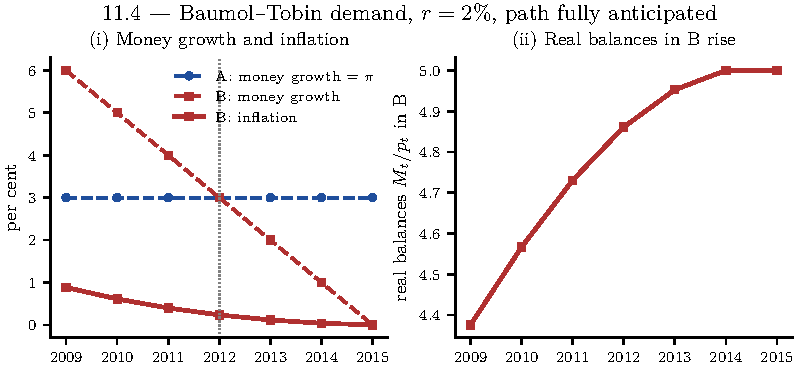
\includegraphics[width=\linewidth]{fig/fig_k11_4_inflation.pdf}\\[3pt]
\captionof{figure}{Problem 11.4. Money growth and inflation in A and B (left); B's real balances (right).}
\label{fig:k11-4}
\end{center}

\begin{tcolorbox}[trapbox]
\small
``Both grow money at 3\% in 2012, so both have 3\% inflation'' applies the steady-state
formula $\pi=\mu$ out of steady state. $\pi=\mu$ holds only when expected inflation, and
hence $i$ and real balances, are constant. Country A is in that position; Country B is not.
\end{tcolorbox}
\end{tcolorbox}

%------- 11.5 -------
% Topic: Inflation in Equilibrium
% Keywords: inflation targeting, level adjustment of money, real interest rate shock
\begin{tcolorbox}[oddbox,title={Problem 11.5 \quad Inflation Targeting}]
\begin{tcolorbox}[questionbox]
(a) Suppose a Central Bank has decided it wants to keep inflation at exactly 2\% every year. The
economy is not growing and the real interest rate is 3\%. Describe what the Central Bank must do
to the money supply to achieve its objective.\\
(b) Suppose the real interest rate suddenly and unexpectedly falls from 3\% to 1\%. How should
the Central Bank respond? Explain in detail.
\end{tcolorbox}

\textbf{Solution:}

\begin{enumerate}
\item With $g=0$, (11.2.3) gives $\pi=\mu$. The Central Bank must
\[
\boxed{\text{grow the money supply at }\mu=2\%\text{ per year: }\Ms_{t+1}=1.02\,\Ms_t.}
\]
\emph{Verification.} The nominal rate is $i=r+\pi=3\%+2\%=5\%$ (exactly
$1.03\times1.02-1=5.06\%$), constant. Real balances $\mD(Y,0.05)$ are constant, so
$p_t=\Ms_t/\mD(Y,0.05)$ grows exactly as $\Ms_t$ does, at 2\%. \checkmark\ The \emph{level}
of $\Ms$ pins the level of $p$; its \emph{growth rate} pins inflation.

\item \textbf{Step 1 --- what the shock does to money demand.} If inflation stays at 2\%, the
nominal rate falls from $3\%+2\%=5\%$ to $1\%+2\%=3\%$. Holding money is cheaper, so real money
demand rises from $\mD(Y,0.05)$ to $\mD(Y,0.03)$.

\textbf{Step 2 --- what happens if the Central Bank does nothing.} The stock $\Ms_t=1.02\,\Ms_{t-1}$
is fixed at the moment of the shock. Then
\[
\frac{p_t}{p_{t-1}}=\frac{\Ms_t/\mD(Y,0.03)}{\Ms_{t-1}/\mD(Y,0.05)}
=1.02\times\frac{\mD(Y,0.05)}{\mD(Y,0.03)}<1.02 .
\]
With Baumol--Tobin demand, $\mD\propto i^{-1/2}$, so the ratio is $\sqrt{0.03/0.05}=0.7746$ and
$p_t/p_{t-1}=1.02\times0.7746=0.790$: a one-off \textbf{deflation of about 21\%}. People try to
build up balances, nobody can, and the value of money rises. The target is missed badly.

\textbf{Step 3 --- the right response: a one-time level increase, then the old growth rate.}
Choose $\Ms_t$ so that $p_t=1.02\,p_{t-1}$:
\[
\Ms_t=1.02\,p_{t-1}\,\mD(Y,0.03)=1.02\,\Ms_{t-1}\,\frac{\mD(Y,0.03)}{\mD(Y,0.05)},
\]
and from then on $\Ms_{t+s}=1.02\,\Ms_{t+s-1}$ again. With Baumol--Tobin,
\[
\frac{\mD(Y,0.03)}{\mD(Y,0.05)}=\sqrt{\frac{0.05}{0.03}}=\sqrt{\tfrac53}=1.2910,
\]
\[
\boxed{\begin{array}{c}\text{a one-time injection of }29.1\%\text{ on top of the 2\% trend,}\\
\text{at the moment of the shock; then 2\% growth as before.}\end{array}}
\]

\textbf{Step 4 --- why this is the whole answer.} After the shock the economy is again in a
steady state with constant $i=3\%$, so real balances are constant and 2\% money growth gives
2\% inflation. Only the \emph{level} of money demand has changed, and a level change in demand
is met by a level change in supply. Keeping 2\% growth without the jump misses the target for
one year (Step 2). Raising the growth rate instead would raise inflation permanently.
Timing matters: the injection must come with the shock, because a delay means a fall in prices
followed by a jump back.
\end{enumerate}

\textbf{Verification.} The code solves the perfect-foresight price path after the shock for a
trial jump $x$, finds by root-finding the $x$ that gives $\pi=2\%$ in the shock year,
$x=1.290994=\sqrt{5/3}$, confirms $\pi=2\%$ in every later year, and finds $\pi=-20.99\%$ with no
jump. \checkmark
\end{tcolorbox}

%---- Topic: Seignorage ----
\subsection{Seignorage}

%------- 11.3 -------
% Topic: Seignorage
% Keywords: seignorage, growth, zero inflation, money multiplier, Baumol-Tobin
\begin{tcolorbox}[oddbox,title={Problem 11.3 \quad Seignorage with Zero Inflation and Growth}]
\begin{tcolorbox}[questionbox]
Suppose an economy is growing at a constant rate $g$, money demand comes from the Baumol-Tobin
model and the money multiplier is $\omega$. Suppose the government wants to maintain zero
inflation. How much seignorage revenue can it obtain as a fraction of GDP? In other words, find
an expression for the level of:
\[
\frac{\MBase_t-\MBase_{t-1}}{p_tY_t}
\]
that is consistent with zero inflation. How does this depend on $g$, $F$ and $\omega$? Why?
[Hint: use the result from Exercise 11.1.]
\end{tcolorbox}

\textbf{Solution:}

\textbf{Step 1 --- what zero inflation pins down.} $\pi=0$ means $p_t=p$ constant and, by the
Fisher equation, $i=r$ constant. Money-market equilibrium in every period:
\[
\Ms_t=p\,\mD(Y_t,r)=p\sqrt{\frac{Y_tF}{2r}} .
\]
The Central Bank must supply exactly this; the base is $\MBase_t=\Ms_t/\omega$.

\textbf{Step 2 --- growth of the base.} With $Y_{t-1}=Y_t/(1+g)$,
\[
\MBase_{t-1}=\frac{p}{\omega}\sqrt{\frac{Y_{t-1}F}{2r}}=\frac{p}{\omega}\sqrt{\frac{Y_tF}{2r}}\,(1+g)^{-1/2}
=\MBase_t\,(1+g)^{-1/2}.
\]
The base grows at $(1+g)^{1/2}-1\approx g/2=\eta g$: this is (11.2.3) with $\pi=0$, $\mu=\eta g$,
and $\eta=\tfrac12$ from Problem 11.1.

\textbf{Step 3 --- revenue over GDP.}
\[
\frac{\MBase_t-\MBase_{t-1}}{pY_t}
=\frac{\MBase_t\left[1-(1+g)^{-1/2}\right]}{pY_t}
=\frac{1}{\omega}\cdot\frac{1}{Y_t}\sqrt{\frac{Y_tF}{2r}}\left[1-(1+g)^{-1/2}\right],
\]
\[
\boxed{\frac{\MBase_t-\MBase_{t-1}}{p_tY_t}=\frac{1}{\omega}\sqrt{\frac{F}{2rY_t}}\,
\Bigl[1-(1+g)^{-1/2}\Bigr]
\;\approx\;\frac{\eta\,g}{\omega}\cdot\frac{\mD(Y_t,r)}{Y_t}
=\frac{g}{2\omega}\sqrt{\frac{F}{2rY_t}} .}
\]
The approximation uses $1-(1+g)^{-1/2}\approx g/2$ for small $g$.

\textbf{Step 4 --- comparative statics and why.}
\begin{itemize}
\item \textbf{Increasing in $g$.} Growth raises the demand for real balances every period, and
the government meets it by issuing new base \emph{without} causing inflation. With no growth
($g=0$) the revenue is zero: every dollar of seignorage then requires inflation (footnote 4 of
the chapter). The hint enters here: revenue is proportional to $\eta g$; with $\eta=1$ it would be
twice as large.
\item \textbf{Increasing in $F$} (as $\sqrt F$). A higher trip cost makes people hold more money
per unit of GDP, $\mD/Y=\sqrt{F/2rY}$. The tax base, and its growth, are larger. Financial
innovation that lowers $F$ erodes the revenue.
\item \textbf{Decreasing in $\omega$} (as $1/\omega$). The government issues only the base. The
rest of M1 is deposits, which private banks create, and the interest saved on them accrues to
banks (Problem 11.7). The larger the multiplier, the smaller the base behind each dollar of M1.
\end{itemize}
One more feature: because $\eta<1$, $\mD/Y\propto Y^{-1/2}$ falls as the economy grows, so the
revenue \emph{share} slowly declines over time even at constant $g$.

\begin{tcolorbox}[databox]
With $g=0.03$, $F=0.02$, $\omega=5$, $r=0.03$, the code builds $Y_t$, $\Ms_t$ and $\MBase_t$
period by period at $p=1$ and matches the exact formula to $10^{-14}$: $0.0015734$ of GDP,
against $0.0016087$ from the first-order approximation (a gap of $2.2\%$, of order $g$). It
also confirms that revenue rises with $g$ and $F$ (a fourfold $F$ doubles it), falls with
$\omega$, and is zero at $g=0$.
\end{tcolorbox}
\end{tcolorbox}

%------- 11.6 -------
% Topic: Seignorage
% Keywords: Cagan money demand, inflation tax Laffer curve, hyperinflation, stabilisation, remonetisation
\begin{tcolorbox}[evenbox,title={Problem 11.6 \quad Seignorage with High Inflation}]
\begin{tcolorbox}[questionbox]
Suppose that money demand is given by:
\[
\mD(Y_t,i_{t+1})=Y_t\cdot(1+i_{t+1})^{-\mu}
\]
where $\mu$ is a parameter. This is sometimes known as the Cagan money-demand function.
Equilibrium in the money market is given by:
\[
\Ms_t=Y_t\cdot(1+i_{t+1})^{-\mu}p_t
\]
The real economy is in a steady state so that $Y_t=Y_{ss}$, $r_{t+1}=r_{ss}$. The government
obtains seignorage revenue $S_t$ (in real terms) by expanding the monetary base. $S_t$ is given by:
\[
S_t=\frac{\MBase_t-\MBase_{t-1}}{P_t}\qquad(11.4.2)
\]
Let $\omega$ be the money multiplier, so that $\Ms=\omega\MBase$. Suppose that the rate of growth
of the money supply is constant at rate $\gamma$, i.e.:
\[
\Ms_t=(1+\gamma)\Ms_{t-1}\qquad(11.4.3)
\]
(a) What will be the rate of inflation?\\
(b) What will be nominal interest rate?\\
(c) Find an expression for the level of real money balances. How does it depend on $\gamma$? Why?\\
(d) Solve equation (11.4.3) for $\Ms_{t-1}$ and replace this in (11.4.2) to obtain an expression
for seignorage revenue $S_t$ in terms of $\gamma$ and $\frac{\Ms_t}{P_t}$. How does $S_t$ depend on
$\gamma$? How does it depend on $\frac{\Ms_t}{P_t}$? Why?\\
(e) Replace the value of $\frac{\Ms_t}{P_t}$ that you found in part (c) into the expression for
$S_t$ that you found in part (d) to obtain an expression for seignorage revenues $S_t$ in terms of
$\gamma$, $Y_{ss}$, $r_{ss}$, $\omega$ and $\mu$.\\
(f) Assume the following parameter values: $Y_{ss}=1$, $\mu=4$, $r_{ss}=0.0025$, $\omega=5$.
Note that $\mu=4$ is close to the value that has been empirically estimated in some high inflation
countries when the time period is one month. To be consistent, $r_{ss}$ should be interpreted as a
monthly real interest rate and $Y_{ss}$ as monthly GDP.\\
(g) Plot $S_t$ against $\gamma$ for values of $\gamma$ between 0 and 0.8.\\
(h) What is the monthly rate of growth of the money supply that maximizes seignorage revenue?
Call this $\gamma^\ast$.
\end{tcolorbox}
\begin{tcolorbox}[questionbox,title={\textit{Question (continued)}}]
(i) Why is seignorage revenue decreasing in $\gamma$ for $\gamma>\gamma^\ast$?\\
(j) What monthly inflation rate does $\gamma=\gamma^\ast$ imply?\\
(k) What monthly nominal interest rate does $\gamma=\gamma^\ast$ imply?\\
(l) What yearly rate of inflation does $\gamma=\gamma^\ast$ imply?\\
(m) What is $\frac{M_t}{P_t}$ if $\gamma=\gamma^\ast$?\\
(n) What is the maximum revenue as a fraction of GDP that the government in this example can
constantly collect from seignorage?\\
(o) Look at the data from Sargent (1982) on the German hyperinflation of the 1920s (you can find
it at the book website). What was the maximum monthly inflation rate that Germany experienced?
How does it compare to $\gamma^\ast$?\\
(p) Suppose that the government is increasing the money supply at a rate $\gamma=\gamma^\ast$, and in
month $t$ it credibly announces that (i) $\MBase_{t+1}$ will not be equal to $\MBase_t(1+\gamma^\ast)$ the
way it would have been if the policy had continued as usual, but it will be some other level
$\bar M$ (maybe higher, maybe lower than $\MBase_t(1+\gamma^\ast)$) (ii) from then on, it will set
$\MBase_{t+s}=\bar M$ for every $s\ge1$ (i.e.\ the money supply will be constant).\\
(q) What will be the rate of inflation from period $t+1$ onwards?\\
(r) What will be the price level $P_{t+1}$ in period $t+1$? (This will depend on the government's
choice of $\bar M$.)\\
Suppose the government sets $\bar M$ at the level that will ensure that $P_{t+1}=P_t$ (i.e.\ the
level that will immediately stop inflation).\\
(s) What value of $\bar M$ will it need to choose? How does it compare to $\MBase_t(1+\gamma^\ast)$?\\
(t) How much seignorage revenue will the government obtain in period $t+1$? How does this level
of seignorage compare to what the government was getting every month before making this change?\\
(u) Look carefully at the timing of the end of hyperinflation in Germany. When exactly did the
money supply stop growing? When exactly did hyperinflation stop? How can we make sense of this?
\end{tcolorbox}

\textbf{Solution:} In this problem $\mu$ is Cagan's parameter, the elasticity of real balances
with respect to $1+i$, not a money growth rate. Money growth is $\gamma$.

\begin{enumerate}
\item \textbf{Guess and verify.} Guess a steady state with constant inflation $\pi$. Then
$i_{t+1}$ is constant, so real balances $\Ms_t/P_t=Y_{ss}(1+i)^{-\mu}$ are constant, and $P_t$
must grow at the same rate as $\Ms_t$:
\[
\frac{P_t}{P_{t-1}}=\frac{\Ms_t}{\Ms_{t-1}}=1+\gamma
\qquad\Longrightarrow\qquad\boxed{\pi=\gamma.}
\]
This is (11.2.3) with $g=0$.

\item Fisher, exactly: $1+i=(1+r_{ss})(1+\pi)$, so
\[
\boxed{i=(1+r_{ss})(1+\gamma)-1\;\approx\;r_{ss}+\gamma.}
\]

\item From the equilibrium condition with $1+i=(1+r_{ss})(1+\gamma)$:
\[
\boxed{\frac{\Ms_t}{P_t}=Y_{ss}\bigl[(1+r_{ss})(1+\gamma)\bigr]^{-\mu},}
\qquad
\frac{\partial\ln(\Ms/P)}{\partial\ln(1+\gamma)}=-\mu<0 .
\]
Real balances \textbf{fall} with $\gamma$. Faster money growth means higher inflation, a higher
nominal rate, a higher opportunity cost of holding money, and so smaller real holdings.

\item From (11.4.3), $\Ms_{t-1}=\Ms_t/(1+\gamma)$; with $\MBase=\Ms/\omega$,
\[
S_t=\frac{\Ms_t-\Ms_{t-1}}{\omega P_t}=\frac{1}{\omega}\left(1-\frac{1}{1+\gamma}\right)\frac{\Ms_t}{P_t}
\;\Longrightarrow\;
\boxed{S_t=\frac{1}{\omega}\cdot\frac{\gamma}{1+\gamma}\cdot\frac{\Ms_t}{P_t}.}
\]
Holding real balances fixed, $S_t$ is \textbf{increasing in $\gamma$}: $\gamma/(1+\gamma)$ is the
share of this period's stock that is newly printed, the \emph{rate} of the inflation tax. It is
\textbf{proportional to $\Ms_t/P_t$}, the \emph{base} of the tax: a given growth rate collects
more when people hold more money. Revenue $=$ rate $\times$ base $\div\,\omega$.

\item Substitute (c) into (d):
\[
\boxed{S=\frac{Y_{ss}}{\omega}\cdot\frac{\gamma}{1+\gamma}\bigl[(1+r_{ss})(1+\gamma)\bigr]^{-\mu}
=\frac{Y_{ss}}{\omega}(1+r_{ss})^{-\mu}\,\gamma\,(1+\gamma)^{-(1+\mu)}.}
\]
Now $\gamma$ raises the rate but shrinks the base.

\item With $Y_{ss}=1$, $\mu=4$, $r_{ss}=0.0025$, $\omega=5$: $(1.0025)^{-4}=0.990062$ and
\[
S(\gamma)=\frac{0.990062}{5}\,\gamma(1+\gamma)^{-5}=0.198012\,\gamma(1+\gamma)^{-5}.
\]

\item See Figure~\ref{fig:k11-6}: an inflation-tax Laffer curve, zero at $\gamma=0$, a single
peak, then slowly declining.

\begin{center}
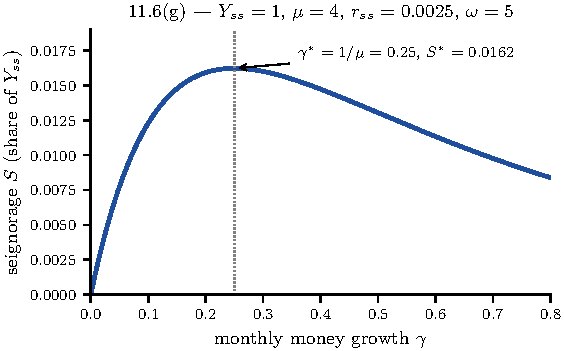
\includegraphics[width=0.68\linewidth]{fig/fig_k11_6_laffer.pdf}\\[3pt]
\captionof{figure}{Problem 11.6(g). Seignorage against monthly money growth.}
\label{fig:k11-6}
\end{center}

\item Maximise $h(\gamma)=\gamma(1+\gamma)^{-(1+\mu)}$ (the constant factor does not move the
argmax):
\[
\begin{aligned}
h'(\gamma)&=(1+\gamma)^{-(1+\mu)}-(1+\mu)\gamma(1+\gamma)^{-(2+\mu)}\\
&=(1+\gamma)^{-(2+\mu)}\bigl[(1+\gamma)-(1+\mu)\gamma\bigr]
=(1+\gamma)^{-(2+\mu)}\,(1-\mu\gamma).
\end{aligned}
\]
Setting it to zero:
\[
\boxed{\gamma^\ast=\frac{1}{\mu}=\frac14=25\%\ \text{per month}.}
\]
$h'>0$ for $\gamma<1/\mu$ and $h'<0$ for $\gamma>1/\mu$, so this is the global maximum.

\item Take logs of (e) and differentiate with respect to $\ln(1+\gamma)$:
\[
\frac{d\ln S}{d\ln(1+\gamma)}
=\underbrace{\frac{d\ln\frac{\gamma}{1+\gamma}}{d\ln(1+\gamma)}}_{\text{rate}:\ 1/\gamma}
\;+\;\underbrace{\frac{d\ln(\Ms/P)}{d\ln(1+\gamma)}}_{\text{base}:\ -\mu}
=\frac1\gamma-\mu ,
\]
where the rate term is $(1+\gamma)\bigl[\tfrac1\gamma-\tfrac1{1+\gamma}\bigr]=\tfrac1\gamma$. For
$\gamma>1/\mu$, $1/\gamma<\mu$: a further rise in money growth raises the tax rate by
proportionally \emph{less} than it shrinks the tax base. People flee money (more trips to the
bank, foreign currency, goods) faster than the government can tax it. This is the Laffer logic
the chapter describes in \S11.3.

\item $\pi=\gamma^\ast=\boxed{25\%\ \text{per month}}$.

\item $i=(1.0025)(1.25)-1=1.253125-1=\boxed{25.31\%\ \text{per month}}$.

\item Compound twelve months: $1.25^2=1.5625$, $1.25^4=2.44140625$, $1.25^8=5.96046448$,
$1.25^{12}=5.96046448\times2.44140625=14.5519152$, so
\[
\boxed{(1.25)^{12}-1=13.55,\ \text{i.e.\ about }1{,}355\%\ \text{per year}.}
\]

\item $1.253125^2=1.57032227$, $1.253125^4=1.57032227^2=2.46591202$, so
\[
\frac{M_t}{P_t}=1\times(1.253125)^{-4}=\frac{1}{2.46591202}=\boxed{0.4055}
\]
(59\% below the $(1.0025)^{-4}=0.990$ held at zero inflation).

\item $S^\ast=\dfrac{1}{5}\cdot\dfrac{0.25}{1.25}\cdot0.405529=0.2\times0.2\times0.405529
=\boxed{0.01622},$ i.e.\ \textbf{1.62\% of GDP} (monthly revenue over monthly GDP), the most the
government can collect month after month.

\item The Sargent (1982) tables are on the book's website and are not in this repository, so
the exact monthly figures are not reproduced here. The magnitude is well documented: at the peak,
in the autumn of 1923, German prices were rising about \textbf{300-fold in a single month}
(Jones, \emph{Macroeconomics}, 2020, ch.~8, drawing on Sargent), i.e.\ monthly inflation near
$29{,}900\%$, against $\gamma^\ast=25\%$: \textbf{roughly 1{,}200 times} the revenue-maximising
rate. Germany was far down the wrong side of the Laffer curve. At such rates real balances are a
tiny fraction of their normal level and steady-state revenue is far below $S^\ast$. Printing that
fast makes sense only as a chase of \emph{transitory} revenue (each acceleration collects more
before money demand adjusts) or as a loss of fiscal control. It cannot be explained as
steady-state revenue maximisation.

\item[(p)] (Set-up of the reform; the questions are (q)--(t).)

\item[(q)] From $t+1$ on, $\MBase$, and so $\Ms=\omega\bar M$, is constant. By (a) with $\gamma=0$:
\[
\boxed{\pi_{t+2}=\pi_{t+3}=\dots=0,\qquad i_{t+2}=r_{ss}.}
\]
Inflation between $t$ and $t+1$ depends on $\bar M$ (parts (r)--(s)).

\item[(r)] Money-market equilibrium in $t+1$, with $1+i_{t+2}=1+r_{ss}$:
\[
\omega\bar M=Y_{ss}(1+r_{ss})^{-\mu}P_{t+1}
\qquad\Longrightarrow\qquad
\boxed{P_{t+1}=\frac{\omega\bar M\,(1+r_{ss})^{\mu}}{Y_{ss}}.}
\]

\item[(s)] \emph{Reading of the timing.} The month-$t$ market has already cleared under the old
expectations (announcement at the end of month $t$), so
$P_t=\omega\MBase_t\bigl[(1+r_{ss})(1+\gamma^\ast)\bigr]^{\mu}/Y_{ss}$. Setting $P_{t+1}=P_t$:
\[
\omega\bar M(1+r_{ss})^{\mu}=\omega\MBase_t(1+r_{ss})^{\mu}(1+\gamma^\ast)^{\mu}
\]
\[
\Longrightarrow\quad
\boxed{\bar M=\MBase_t(1+\gamma^\ast)^{\mu}=1.25^4\,\MBase_t=2.441\,\MBase_t.}
\]
Compared with the business-as-usual $\MBase_t(1+\gamma^\ast)=1.25\,\MBase_t$, the ratio is
$(1+\gamma^\ast)^{\mu-1}=1.25^3=1.953$. To \textbf{stop} inflation the government must print
\textbf{almost twice as much} as it would have printed to \emph{continue} it. The reason is that
ending inflation drops the nominal rate from 25.3\% to 0.25\% a month, so real money demand
jumps by the factor $1.25^4=2.44$ (remonetisation). At constant prices, that extra demand can
only be met with extra nominal money. If the government printed less, $P_{t+1}$ would
\emph{fall}.

\item[(t)]
\[
S_{t+1}=\frac{\bar M-\MBase_t}{P_{t+1}}=\frac{\MBase_t}{P_t}\bigl[(1+\gamma^\ast)^{\mu}-1\bigr]
\]
\[
=\frac{0.405529}{5}\times(2.44140625-1)=0.081106\times1.44140625=\boxed{0.1169},
\]
using $P_{t+1}=P_t$ and $\MBase_t/P_t=(\Ms_t/P_t)/\omega$. That is \textbf{11.7\% of monthly GDP},
$0.1169/0.01622=\mathbf{7.21}$ times the steady-state maximum $S^\ast$ (exactly
$(1+\gamma^\ast)\bigl[(1+\gamma^\ast)^\mu-1\bigr]/\gamma^\ast=1.25\times1.4414/0.25$). It is a
one-off: from $t+2$ on revenue is zero. A credible stabilisation hands the government a single
large seignorage payment, collected from the public's rebuilding of its real balances.

\begin{center}
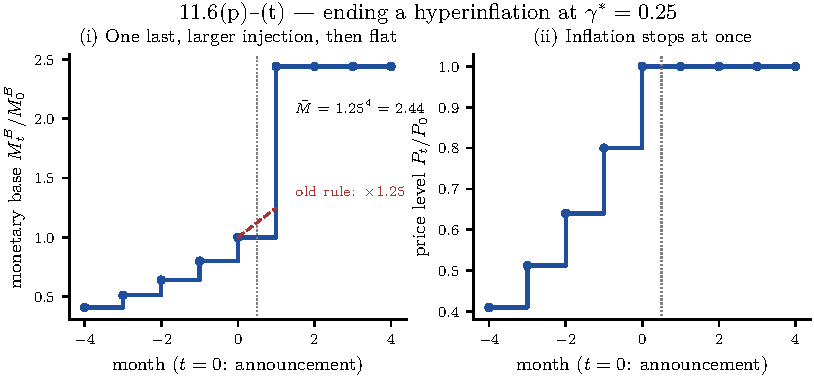
\includegraphics[width=\linewidth]{fig/fig_k11_6_stabilisation.pdf}\\[3pt]
\captionof{figure}{Problem 11.6(p)--(t). The base jumps to $\bar M=2.44\,\MBase_t$ and stays
there; the price level stops rising at once.}
\label{fig:k11-6b}
\end{center}

\item[(u)] Sargent's reading of the German episode (and of the other interwar
hyperinflations) is that inflation ended \textbf{abruptly} in November 1923, with the currency
reform and a credible fiscal reform, while the stock of central-bank money \textbf{kept growing
substantially for months afterwards}. Prices stopped before money did. The model explains the
timing. Once the regime change is credible, expected inflation collapses, the nominal rate falls,
and the demand for real balances multiplies, by $1.25^4$ in our calibration and by far more from
German inflation rates. Large nominal injections after stabilisation are then exactly what
\emph{keeps} prices stable: they meet the remonetisation demand of part (s). What had to stop at
once was the expected \emph{future} path of money (fiscal credibility), not the current
printing.
\end{enumerate}

\begin{tcolorbox}[databox]
The code builds $\Ms_t$, $\MBase_t$ and $P_t$ from the definitions and matches (e) to
$10^{-14}$; a bounded optimiser and an 800{,}001-point grid both return $\gamma^\ast=0.250000$.
It prints $i=0.253125$, $1.25^{12}-1=13.5519$, $M/P=0.405529$, $S^\ast=0.016221$; the base
elasticity $-4$ and rate elasticity $1/\gamma^\ast=4$ at the peak by finite differences; and, by
root-finding on $P_{t+1}=P_t$, $\bar M=2.441406\,\MBase_t$, $S_{t+1}=0.116907$ and the ratio $7.2070$.
\end{tcolorbox}

\begin{tcolorbox}[trapbox]
\small
\textbf{The timing in (s) is a reading, not a given.} If the announcement came \emph{before}
the month-$t$ market cleared, then $i_{t+1}$ would already reflect zero expected inflation, $P_t$
itself would fall on the announcement (to $\omega\MBase_t(1+r_{ss})^{\mu}/Y_{ss}$), and
$P_{t+1}=P_t$ would require $\bar M=\MBase_t$: no extra money at all. The question's comparison with
$\MBase_t(1+\gamma^\ast)$ and part (u) point to the reading used above, where $P_t$ is already set
under the old regime.

\smallskip
Also: (q) asks about inflation ``from $t+1$ onwards''. Inflation between $t+1$ and later months is
zero whatever $\bar M$ is; inflation \emph{into} $t+1$ is what $\bar M$ controls.
\end{tcolorbox}
\end{tcolorbox}

%------- 11.7 -------
% Topic: Seignorage
% Keywords: bank seignorage, deposits, interest-inelastic margin, M1 data
\begin{tcolorbox}[oddbox,title={Problem 11.7 \quad Bank Seignorage}]
\begin{tcolorbox}[questionbox]
Suppose that the demand for M1 money is given by $\frac{M}{pY}=A-\eta i$ where $M$ is the
quantity of M1 money, $pY$ is nominal GDP, $i$ is the nominal interest rate and $A$ and $\eta$
are parameters. Households want to hold a fraction $\chi$ of their M1 money in the form of cash and
a fraction $1-\chi$ in the form of checking accounts, which earn no interest. Banks earn seignorage
by taking checking deposits and investing in assets that earn the nominal interest rate.\\[3pt]
(a) Find an expression for the ratio of total seignorage earned by banks to GDP. Call this ratio $s$.\\
(b) Compute $\frac{\partial s}{\partial i}$. Why does this number depend on $\eta$?\\
(c) Look up data on M1 and its components in 2018. What is a reasonable value for $\chi$? What
was the value of $\frac{M}{pY}$? If the average nominal interest was 2\%, how much seignorage did
banks earn as a fraction of GDP?\\
(d) If $\eta=0.2$, how much seignorage would banks earn as a fraction of GDP if the nominal
interest rate went up to 3\%?
\end{tcolorbox}

\textbf{Solution:} As in the statement, banks invest the whole deposit base at $i$ (no reserves;
with a reserve ratio $\rho$ earning nothing, multiply every expression by $1-\rho$). Note that
$\eta$ here is the semi-elasticity in $A-\eta i$, not the income elasticity of \S11.2.

\begin{enumerate}
\item Deposits are $D=(1-\chi)M$. Banks pay zero on them and earn $i$, so bank seignorage is
$iD=i(1-\chi)M$. Dividing by $pY$ and substituting the demand function:
\[
\boxed{s=\frac{i(1-\chi)M}{pY}=i\,(1-\chi)\,(A-\eta i).}
\]

\item
\[
\boxed{\pd{s}{i}=(1-\chi)\bigl[(A-\eta i)+i(-\eta)\bigr]=(1-\chi)(A-2\eta i).}
\]
A higher $i$ has two effects. It raises the margin on every deposit dollar (the term
$A-\eta i$, the current base), and it shrinks the base, because people hold less M1 when its
opportunity cost rises (the term $-\eta i$). $\eta$ measures how fast the base shrinks. With
$\eta=0$, bank seignorage would be linear in $i$; with $\eta>0$ it is a Laffer curve in $i$
with peak at $i=A/(2\eta)$, the same logic as Problem 11.6.

\item \emph{Data (approximate, US, 2018, FRED series \texttt{CURRSL}, \texttt{M1SL}, \texttt{GDP};
pre-2020 M1 definition).} Currency $\approx\$1.63$ trillion, M1 $\approx\$3.75$ trillion,
nominal GDP $\approx\$20.6$ trillion. Then
\[
\chi\approx\frac{1.63}{3.75}=\boxed{0.43},\qquad
\frac{M}{pY}\approx\frac{3.75}{20.6}=\boxed{0.18},
\]
\[
s=0.02\times(1-0.435)\times0.182=\boxed{0.0021},\ \text{about }0.2\%\text{ of GDP}
\ (\approx\$42\ \text{billion}).
\]
Caveats: a large share of US currency is held abroad, so $\chi$ overstates domestic cash
use; and some checkable deposits do pay a little interest, which lowers the true margin.

\item Calibrate $A$ from (c): $A=M/pY+\eta i=0.1820+0.2\times0.02=0.1860$. At $i=3\%$:
\[
\frac{M}{pY}=0.1860-0.2\times0.03=0.1800,\qquad
s=0.03\times0.565\times0.1800=\boxed{0.0031},
\]
about \textbf{0.31\% of GDP}, 48\% more than at 2\%. The base shrinks only 1.1\%, and the margin
rises 50\%, because $i=3\%$ is far below the peak $A/2\eta=46.5\%$.
\end{enumerate}

\textbf{Verification.} The code builds $M$, $D$ and interest income in levels and matches (a);
the finite-difference derivative matches (b); it reproduces $\chi=0.435$, $M/pY=0.1820$,
$s(2\%)=0.00206$, $A=0.18604$ and $s(3\%)=0.00305$ (ratio $1.4835$). \checkmark
\end{tcolorbox}

%---- Topic: Real Interest Rates ----
\subsection{Real Interest Rates}

%------- 11.8 -------
% Topic: Real Interest Rates
% Keywords: Fisher equation, unexpected inflation, redistribution, borrowers and lenders
\begin{tcolorbox}[evenbox,title={Problem 11.8 \quad Real Interest Rates}]
\begin{tcolorbox}[questionbox]
Define realized real interest rates $r_{t+1}$ as:
\[
r_{t+1}\equiv i_{t+1}-\pi_{t+1}
\]
where $i_{t+1}$ is the nominal interest rate between period $t$ and period $t+1$ and $\pi_{t+1}$ is
the rate of inflation between period $t$ and period $t+1$. If there is uncertainty about what the
rate of inflation is going to be, this implies that there is uncertainty about what realized real
interest rates will be. Define the expected real interest rate as:
\[
r^E_{t+1}\equiv i_{t+1}-E(\pi_{t+1})
\]
where $E(\pi_{t+1})$ is the expected rate of inflation. Suppose there are two parties to a nominal
lending contract: a borrower and a lender. Who benefits when realized real interest rates turn out
to be higher than expected real interest rates? What monetary policy will each of them support?
\end{tcolorbox}

\textbf{Solution:}

\textbf{Step 1 --- the gap.} The nominal rate $i_{t+1}$ is fixed in the contract, so subtracting
the two definitions,
\[
r_{t+1}-r^E_{t+1}=\bigl(i_{t+1}-\pi_{t+1}\bigr)-\bigl(i_{t+1}-E(\pi_{t+1})\bigr)=E(\pi_{t+1})-\pi_{t+1}.
\]
Realized real rates exceed expected ones exactly when \textbf{inflation turns out lower than
expected}.

\textbf{Step 2 --- who gains.} Per unit of goods lent, the lender receives a real return
$r_{t+1}$ and the borrower pays that same $r_{t+1}$. The contract was priced on $r^E_{t+1}$. When
$r_{t+1}>r^E_{t+1}$ the lender gets more goods back than bargained for, and the borrower repays
more goods than bargained for:
\[
\boxed{\text{the \textbf{lender} gains and the \textbf{borrower} loses, each by }E(\pi_{t+1})-\pi_{t+1}
\text{ per unit lent.}}
\]
Example: $i=6\%$, $E(\pi)=3\%$, so $r^E=3\%$. If $\pi=1\%$, $r=5\%$: the lender earns 2
extra cents per real dollar and the borrower pays them. If $\pi=5\%$, $r=1\%$ and the transfer
reverses.

\textbf{Step 3 --- policy preferences.} Only \emph{unexpected} inflation redistributes; expected
inflation is already in $i$.
\begin{itemize}
\item \textbf{Lenders} (creditors, bondholders, savers in nominal assets) gain from inflation
below expectations and lose from surprises above. They favour a tight, anti-inflationary
central bank, and at the very least one that never lets inflation exceed what was priced in.
\item \textbf{Borrowers} (debtors with fixed-rate nominal debt, including governments) gain from
inflation above expectations, which erodes the real value of their repayments. They favour
looser policy and higher-than-expected inflation.
\end{itemize}
Both sides have the same interest \emph{ex ante} in predictable inflation, which lowers the risk
on either side of the contract. The conflict arises \emph{ex post}, once the contracts are signed.
\end{tcolorbox}

%---- Topic: Money in Practice ----
\subsection{Money in Practice}

%------- 11.9 -------
% Topic: Money in Practice
% Keywords: commodity money, quantity theory, Radford 1945, cigarette currency
\begin{tcolorbox}[oddbox,title={Problem 11.9 \quad Money among Prisoners of War}]
\begin{tcolorbox}[questionbox]
Read ``The Economic Organisation of a P.O.W. Camp'', which you can find at:
\url{https://www.jstor.org/stable/2550133}. Pick one passage out of the article and explain how it
relates to the models of money supply, money demand and inflation from Chapters 10 and 11.
\end{tcolorbox}

\textbf{Solution:} The article (Radford, \emph{Economica}, 1945) is not in this repository, so
the passage is \emph{paraphrased} below, not quoted; the reader should check the wording against
the original.

\textbf{The passage.} Radford describes how cigarettes became the camp's money, and how the
general level of prices, measured in cigarettes, rose and fell with the supply of cigarettes.
When a large delivery of Red Cross parcels or private cigarette consignments arrived, prices
rose. As the week went on and cigarettes were smoked, prices fell. Long interruptions in the
supply of cigarettes produced a general deflation.

\textbf{Mapping onto Chapters 10--11.}
\begin{enumerate}
\item \emph{Money supply.} The camp's money stock $\Ms$ is the stock of cigarettes held for
exchange. No authority controls it: it rises with deliveries (an ``open market operation''
by the Red Cross) and \emph{shrinks through consumption}, since smoking a cigarette destroys
money. Commodity money has an intrinsic use that competes with its monetary role.
\item \emph{Money demand.} Real demand $\mD(Y,i)$ depends on the volume of transactions (the
goods in the parcels being traded) and on the cost of holding cigarettes as money instead of
smoking them. That cost plays the role of the forgone interest $i$ in Baumol--Tobin. Within a
parcel cycle the volume of goods to trade is roughly fixed, so real demand is roughly stable.
\item \emph{Price level.} With stable real demand and a flexible price system, (11.2.2) gives
$p=\Ms/\mD(Y,i)$: the camp's price level moves in proportion to its money stock. A delivery is a
one-time increase in $\Ms$ and prices jump (\S11.2, one-time increase in the money supply).
Smoking during the week is a steady \emph{negative} $\mu$ and gives steady deflation,
$\pi\approx\mu$ in (11.2.3) with $g\approx0$. This is the quantity theory working in the most
transparent laboratory one could design, with flexible prices and no interest-bearing assets
to muddy velocity.
\item \emph{A further link.} The same article describes how cigarettes of worse quality
circulated as money while better ones were smoked (Gresham's law). The \emph{quality} of the
money stock, not only its quantity, reacted to the incentive to use the good-for-smoking unit
as a good, not as money.
\end{enumerate}
\end{tcolorbox}

%======================================================================
\section*{Companion code}
\addcontentsline{toc}{section}{Companion code}
%======================================================================

Every numerical result above is reproduced by \texttt{Resolucao/kurlat\_ch10-11\_codigo/}. Each
script checks its analytical formulas against an independent numerical computation and aborts on
any mismatch.

\begin{center}
\begin{tabular}{@{}lp{10.2cm}@{}}
\toprule
\textbf{File} & \textbf{What it does} \\
\midrule
\texttt{ch10\_11\_numerico.py} & 10.1--10.3: a round-by-round deposit chain against (10.3.1), the
finite-difference derivatives in $\rho$ and $\chi$, the table of Problem 10.2 and the divergence
of $\omega$. 10.4--10.5: Baumol--Tobin by numerical minimisation and root-finding. 11.1:
$\eta$ by finite differences. 11.3: period-by-period base against the closed form. 11.4 and
11.5: perfect-foresight price paths solved backwards by root-finding. 11.6: seignorage built from
the definitions, the argmax by optimiser and grid, all of (h)--(n), and $\bar M$ and $S_{t+1}$ by
root-finding. 11.7: levels against the formula, the derivative, the 2018 numbers. 11.8: the
sign of the transfer. \\
\texttt{ch10\_11\_figuras.py} & The three figures. \\
\texttt{estilo\_mpl.py} & \texttt{pgf} backend, so figure text is typeset by \texttt{pdflatex}
with \texttt{lmodern} and \texttt{cmap} and the PDF stays fully copyable. \\
\bottomrule
\end{tabular}
\end{center}

\end{document}
